% Created by tikzDevice version 0.12.3 on 2020-05-27 21:28:00
% !TEX encoding = UTF-8 Unicode
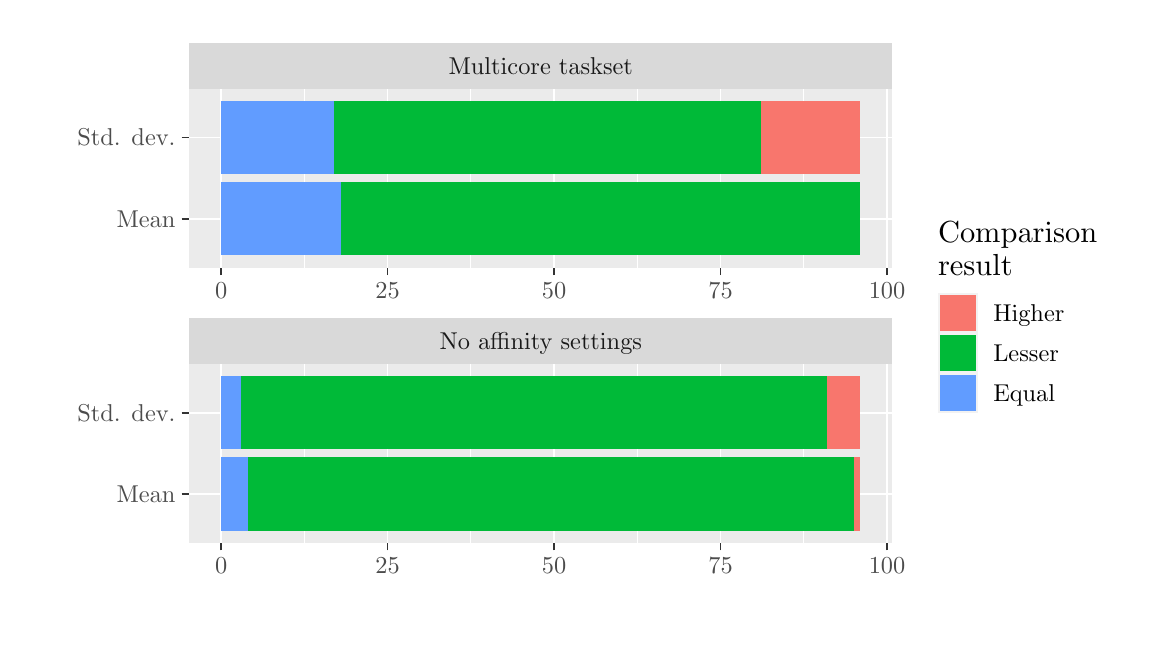
\begin{tikzpicture}[x=1pt,y=1pt]
\definecolor{fillColor}{RGB}{255,255,255}
\path[use as bounding box,fill=fillColor,fill opacity=0.00] (0,0) rectangle (397.48,216.81);
\begin{scope}
\path[clip] (  0.00,  0.00) rectangle (397.48,216.81);
\definecolor{drawColor}{RGB}{255,255,255}
\definecolor{fillColor}{RGB}{255,255,255}

\path[draw=drawColor,line width= 0.6pt,line join=round,line cap=round,fill=fillColor] (  0.00,  0.00) rectangle (397.48,216.81);
\end{scope}
\begin{scope}
\path[clip] ( 58.35,130.11) rectangle (312.46,194.74);
\definecolor{fillColor}{gray}{0.92}

\path[fill=fillColor] ( 58.35,130.11) rectangle (312.46,194.74);
\definecolor{drawColor}{RGB}{255,255,255}

\path[draw=drawColor,line width= 0.3pt,line join=round] ( 99.98,130.11) --
	( 99.98,194.74);

\path[draw=drawColor,line width= 0.3pt,line join=round] (160.14,130.11) --
	(160.14,194.74);

\path[draw=drawColor,line width= 0.3pt,line join=round] (220.30,130.11) --
	(220.30,194.74);

\path[draw=drawColor,line width= 0.3pt,line join=round] (280.46,130.11) --
	(280.46,194.74);

\path[draw=drawColor,line width= 0.6pt,line join=round] ( 58.35,147.73) --
	(312.46,147.73);

\path[draw=drawColor,line width= 0.6pt,line join=round] ( 58.35,177.11) --
	(312.46,177.11);

\path[draw=drawColor,line width= 0.6pt,line join=round] ( 69.90,130.11) --
	( 69.90,194.74);

\path[draw=drawColor,line width= 0.6pt,line join=round] (130.06,130.11) --
	(130.06,194.74);

\path[draw=drawColor,line width= 0.6pt,line join=round] (190.22,130.11) --
	(190.22,194.74);

\path[draw=drawColor,line width= 0.6pt,line join=round] (250.38,130.11) --
	(250.38,194.74);

\path[draw=drawColor,line width= 0.6pt,line join=round] (310.54,130.11) --
	(310.54,194.74);
\definecolor{fillColor}{RGB}{0,186,56}

\path[fill=fillColor] (113.22,134.52) rectangle (300.91,160.95);
\definecolor{fillColor}{RGB}{97,156,255}

\path[fill=fillColor] ( 69.90,134.52) rectangle (113.22,160.95);
\definecolor{fillColor}{RGB}{248,118,109}

\path[fill=fillColor] (264.82,163.89) rectangle (300.91,190.33);
\definecolor{fillColor}{RGB}{0,186,56}

\path[fill=fillColor] (110.81,163.89) rectangle (264.82,190.33);
\definecolor{fillColor}{RGB}{97,156,255}

\path[fill=fillColor] ( 69.90,163.89) rectangle (110.81,190.33);
\end{scope}
\begin{scope}
\path[clip] ( 58.35, 30.69) rectangle (312.46, 95.32);
\definecolor{fillColor}{gray}{0.92}

\path[fill=fillColor] ( 58.35, 30.69) rectangle (312.46, 95.32);
\definecolor{drawColor}{RGB}{255,255,255}

\path[draw=drawColor,line width= 0.3pt,line join=round] ( 99.98, 30.69) --
	( 99.98, 95.32);

\path[draw=drawColor,line width= 0.3pt,line join=round] (160.14, 30.69) --
	(160.14, 95.32);

\path[draw=drawColor,line width= 0.3pt,line join=round] (220.30, 30.69) --
	(220.30, 95.32);

\path[draw=drawColor,line width= 0.3pt,line join=round] (280.46, 30.69) --
	(280.46, 95.32);

\path[draw=drawColor,line width= 0.6pt,line join=round] ( 58.35, 48.31) --
	(312.46, 48.31);

\path[draw=drawColor,line width= 0.6pt,line join=round] ( 58.35, 77.69) --
	(312.46, 77.69);

\path[draw=drawColor,line width= 0.6pt,line join=round] ( 69.90, 30.69) --
	( 69.90, 95.32);

\path[draw=drawColor,line width= 0.6pt,line join=round] (130.06, 30.69) --
	(130.06, 95.32);

\path[draw=drawColor,line width= 0.6pt,line join=round] (190.22, 30.69) --
	(190.22, 95.32);

\path[draw=drawColor,line width= 0.6pt,line join=round] (250.38, 30.69) --
	(250.38, 95.32);

\path[draw=drawColor,line width= 0.6pt,line join=round] (310.54, 30.69) --
	(310.54, 95.32);
\definecolor{fillColor}{RGB}{248,118,109}

\path[fill=fillColor] (298.51, 35.09) rectangle (300.91, 61.53);
\definecolor{fillColor}{RGB}{0,186,56}

\path[fill=fillColor] ( 79.53, 35.09) rectangle (298.51, 61.53);
\definecolor{fillColor}{RGB}{97,156,255}

\path[fill=fillColor] ( 69.90, 35.09) rectangle ( 79.53, 61.53);
\definecolor{fillColor}{RGB}{248,118,109}

\path[fill=fillColor] (288.88, 64.47) rectangle (300.91, 90.91);
\definecolor{fillColor}{RGB}{0,186,56}

\path[fill=fillColor] ( 77.12, 64.47) rectangle (288.88, 90.91);
\definecolor{fillColor}{RGB}{97,156,255}

\path[fill=fillColor] ( 69.90, 64.47) rectangle ( 77.12, 90.91);
\end{scope}
\begin{scope}
\path[clip] ( 58.35, 95.32) rectangle (312.46,111.89);
\definecolor{fillColor}{gray}{0.85}

\path[fill=fillColor] ( 58.35, 95.32) rectangle (312.46,111.89);
\definecolor{drawColor}{gray}{0.10}

\node[text=drawColor,anchor=base,inner sep=0pt, outer sep=0pt, scale=  0.88] at (185.41,100.57) {No affinity settings};
\end{scope}
\begin{scope}
\path[clip] ( 58.35,194.74) rectangle (312.46,211.31);
\definecolor{fillColor}{gray}{0.85}

\path[fill=fillColor] ( 58.35,194.74) rectangle (312.46,211.31);
\definecolor{drawColor}{gray}{0.10}

\node[text=drawColor,anchor=base,inner sep=0pt, outer sep=0pt, scale=  0.88] at (185.41,199.99) {Multicore taskset};
\end{scope}
\begin{scope}
\path[clip] (  0.00,  0.00) rectangle (397.48,216.81);
\definecolor{drawColor}{gray}{0.20}

\path[draw=drawColor,line width= 0.6pt,line join=round] ( 69.90, 27.94) --
	( 69.90, 30.69);

\path[draw=drawColor,line width= 0.6pt,line join=round] (130.06, 27.94) --
	(130.06, 30.69);

\path[draw=drawColor,line width= 0.6pt,line join=round] (190.22, 27.94) --
	(190.22, 30.69);

\path[draw=drawColor,line width= 0.6pt,line join=round] (250.38, 27.94) --
	(250.38, 30.69);

\path[draw=drawColor,line width= 0.6pt,line join=round] (310.54, 27.94) --
	(310.54, 30.69);
\end{scope}
\begin{scope}
\path[clip] (  0.00,  0.00) rectangle (397.48,216.81);
\definecolor{drawColor}{gray}{0.30}

\node[text=drawColor,anchor=base,inner sep=0pt, outer sep=0pt, scale=  0.88] at ( 69.90, 19.68) {0};

\node[text=drawColor,anchor=base,inner sep=0pt, outer sep=0pt, scale=  0.88] at (130.06, 19.68) {25};

\node[text=drawColor,anchor=base,inner sep=0pt, outer sep=0pt, scale=  0.88] at (190.22, 19.68) {50};

\node[text=drawColor,anchor=base,inner sep=0pt, outer sep=0pt, scale=  0.88] at (250.38, 19.68) {75};

\node[text=drawColor,anchor=base,inner sep=0pt, outer sep=0pt, scale=  0.88] at (310.54, 19.68) {100};
\end{scope}
\begin{scope}
\path[clip] (  0.00,  0.00) rectangle (397.48,216.81);
\definecolor{drawColor}{gray}{0.20}

\path[draw=drawColor,line width= 0.6pt,line join=round] ( 69.90,127.36) --
	( 69.90,130.11);

\path[draw=drawColor,line width= 0.6pt,line join=round] (130.06,127.36) --
	(130.06,130.11);

\path[draw=drawColor,line width= 0.6pt,line join=round] (190.22,127.36) --
	(190.22,130.11);

\path[draw=drawColor,line width= 0.6pt,line join=round] (250.38,127.36) --
	(250.38,130.11);

\path[draw=drawColor,line width= 0.6pt,line join=round] (310.54,127.36) --
	(310.54,130.11);
\end{scope}
\begin{scope}
\path[clip] (  0.00,  0.00) rectangle (397.48,216.81);
\definecolor{drawColor}{gray}{0.30}

\node[text=drawColor,anchor=base,inner sep=0pt, outer sep=0pt, scale=  0.88] at ( 69.90,119.10) {0};

\node[text=drawColor,anchor=base,inner sep=0pt, outer sep=0pt, scale=  0.88] at (130.06,119.10) {25};

\node[text=drawColor,anchor=base,inner sep=0pt, outer sep=0pt, scale=  0.88] at (190.22,119.10) {50};

\node[text=drawColor,anchor=base,inner sep=0pt, outer sep=0pt, scale=  0.88] at (250.38,119.10) {75};

\node[text=drawColor,anchor=base,inner sep=0pt, outer sep=0pt, scale=  0.88] at (310.54,119.10) {100};
\end{scope}
\begin{scope}
\path[clip] (  0.00,  0.00) rectangle (397.48,216.81);
\definecolor{drawColor}{gray}{0.30}

\node[text=drawColor,anchor=base east,inner sep=0pt, outer sep=0pt, scale=  0.88] at ( 53.40,144.70) {Mean};

\node[text=drawColor,anchor=base east,inner sep=0pt, outer sep=0pt, scale=  0.88] at ( 53.40,174.08) {Std. dev.};
\end{scope}
\begin{scope}
\path[clip] (  0.00,  0.00) rectangle (397.48,216.81);
\definecolor{drawColor}{gray}{0.20}

\path[draw=drawColor,line width= 0.6pt,line join=round] ( 55.60,147.73) --
	( 58.35,147.73);

\path[draw=drawColor,line width= 0.6pt,line join=round] ( 55.60,177.11) --
	( 58.35,177.11);
\end{scope}
\begin{scope}
\path[clip] (  0.00,  0.00) rectangle (397.48,216.81);
\definecolor{drawColor}{gray}{0.30}

\node[text=drawColor,anchor=base east,inner sep=0pt, outer sep=0pt, scale=  0.88] at ( 53.40, 45.28) {Mean};

\node[text=drawColor,anchor=base east,inner sep=0pt, outer sep=0pt, scale=  0.88] at ( 53.40, 74.66) {Std. dev.};
\end{scope}
\begin{scope}
\path[clip] (  0.00,  0.00) rectangle (397.48,216.81);
\definecolor{drawColor}{gray}{0.20}

\path[draw=drawColor,line width= 0.6pt,line join=round] ( 55.60, 48.31) --
	( 58.35, 48.31);

\path[draw=drawColor,line width= 0.6pt,line join=round] ( 55.60, 77.69) --
	( 58.35, 77.69);
\end{scope}
\begin{scope}
\path[clip] (  0.00,  0.00) rectangle (397.48,216.81);
\definecolor{fillColor}{RGB}{255,255,255}

\path[fill=fillColor] (323.46, 71.98) rectangle (391.98,153.44);
\end{scope}
\begin{scope}
\path[clip] (  0.00,  0.00) rectangle (397.48,216.81);
\definecolor{drawColor}{RGB}{0,0,0}

\node[text=drawColor,anchor=base west,inner sep=0pt, outer sep=0pt, scale=  1.10] at (328.96,139.30) {Comparison};

\node[text=drawColor,anchor=base west,inner sep=0pt, outer sep=0pt, scale=  1.10] at (328.96,127.42) {result};
\end{scope}
\begin{scope}
\path[clip] (  0.00,  0.00) rectangle (397.48,216.81);
\definecolor{fillColor}{gray}{0.95}

\path[fill=fillColor] (328.96,106.39) rectangle (343.42,120.85);
\end{scope}
\begin{scope}
\path[clip] (  0.00,  0.00) rectangle (397.48,216.81);
\definecolor{fillColor}{RGB}{248,118,109}

\path[fill=fillColor] (329.67,107.10) rectangle (342.71,120.13);
\end{scope}
\begin{scope}
\path[clip] (  0.00,  0.00) rectangle (397.48,216.81);
\definecolor{fillColor}{gray}{0.95}

\path[fill=fillColor] (328.96, 91.94) rectangle (343.42,106.39);
\end{scope}
\begin{scope}
\path[clip] (  0.00,  0.00) rectangle (397.48,216.81);
\definecolor{fillColor}{RGB}{0,186,56}

\path[fill=fillColor] (329.67, 92.65) rectangle (342.71,105.68);
\end{scope}
\begin{scope}
\path[clip] (  0.00,  0.00) rectangle (397.48,216.81);
\definecolor{fillColor}{gray}{0.95}

\path[fill=fillColor] (328.96, 77.48) rectangle (343.42, 91.94);
\end{scope}
\begin{scope}
\path[clip] (  0.00,  0.00) rectangle (397.48,216.81);
\definecolor{fillColor}{RGB}{97,156,255}

\path[fill=fillColor] (329.67, 78.20) rectangle (342.71, 91.23);
\end{scope}
\begin{scope}
\path[clip] (  0.00,  0.00) rectangle (397.48,216.81);
\definecolor{drawColor}{RGB}{0,0,0}

\node[text=drawColor,anchor=base west,inner sep=0pt, outer sep=0pt, scale=  0.88] at (348.92,110.59) {Higher};
\end{scope}
\begin{scope}
\path[clip] (  0.00,  0.00) rectangle (397.48,216.81);
\definecolor{drawColor}{RGB}{0,0,0}

\node[text=drawColor,anchor=base west,inner sep=0pt, outer sep=0pt, scale=  0.88] at (348.92, 96.13) {Lesser};
\end{scope}
\begin{scope}
\path[clip] (  0.00,  0.00) rectangle (397.48,216.81);
\definecolor{drawColor}{RGB}{0,0,0}

\node[text=drawColor,anchor=base west,inner sep=0pt, outer sep=0pt, scale=  0.88] at (348.92, 81.68) {Equal};
\end{scope}
\end{tikzpicture}
